\documentclass[a4paper,11pt]{report}
\usepackage{chuan_math_gkt}
\usetikzlibrary{angles,quotes,intersections,patterns,decorations.pathreplacing}
\chuanexamsetup

\begin{document}
\examfontsize

\examsecret{绝密$\bigstar$启用前}

\examtitle{2023年普通高等学校招生全国统一考试（全国甲卷理科）}{数\quad 学}

\noticetitle
\begin{examnotice}
\item 答卷前，考生务必将自己的姓名、准考证号填写在答题卡上. 
\item 回答选择题时，选出每小题的答案后，用铅笔把答题卡上对应题目的答案标号涂黑. 如需改动，用橡皮擦干净后，再选涂其他答案标号. 回答非选择题时，将答案写在答题卡上. 写在本试卷上无效. 
\item 考试结束后，将本试卷和答题卡一并交回. 
\end{examnotice}

\examsection{一、选择题：本题共12小题，每小题5分，共60分. 在每小题给出的四个选项中，只有一项是符合题目要求的. }
\begin{examquestions}
\item 设集合$A=\{x\mid x=3k+1,k\in\mathbb Z\}$，$B=\{x\mid x=3k+2,k\in\mathbb Z\}$，$U$为整数集，则$\complement_U(A\cup B)=$
\twochoices{$\{x\mid x=3k,k\in\mathbb Z\}$}{$\{x\mid x=3k-1,k\in\mathbb Z\}$}{$\{x\mid x=3k-2,k\in\mathbb Z\}$}{$\varnothing$}

\item 若复数$(a+\mathrm{i})(1-a\mathrm{i})=2$，$a\in\mathbb R$，则$a=$
\fourchoices{$-1$}{$0$}{$1$}{$2$}

\item 执行下面的程序框图，输出的$B=$
\begin{tightcenter}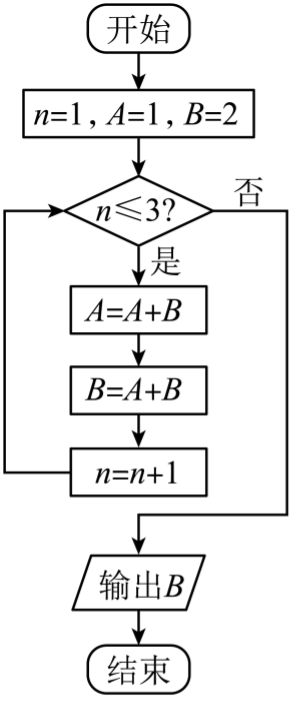
\includegraphics[width=2.3cm]{figures/2023_jia_li_q3.png}\end{tightcenter}
\fourchoices{$21$}{$34$}{$55$}{$89$}
\newpage
\item 向量$|\vec a|=|\vec b|=1$，$|\vec c|=\sqrt2$，且$\vec a+\vec b+\vec c=0$，则$\cos\langle\vec a-\vec c,\vec b-\vec c\rangle=$
\fourchoices{\tallchoice{$-\dfrac15$}}{\tallchoice{$-\dfrac25$}}{\tallchoice{$\dfrac25$}}{\tallchoice{$\dfrac45$}}

\item 已知正项等比数列$\{a_n\}$中，$a_1=1$，$S_n$为$\{a_n\}$前$n$项和，$S_5=5S_3-4$，则$S_4=$
\fourchoices{$7$}{$9$}{$15$}{$30$}

\item 有$50$人报名足球俱乐部，$60$人报名乒乓球俱乐部，$70$人报名足球或乒乓球俱乐部，若已知某人报足球俱乐部，则其报乒乓球俱乐部的概率为
\fourchoices{$0.8$}{$0.4$}{$0.2$}{$0.1$}

\item “$\sin^2\alpha+\sin^2\beta=1$”是“$\sin\alpha+\cos\beta=0$”的
\twochoices{充分条件但不是必要条件}{必要条件但不是充分条件}{充要条件}{既不是充分条件也不是必要条件}

\item 已知双曲线$\dfrac{x^2}{a^2}-\dfrac{y^2}{b^2}=1(a>0,b>0)$的离心率为$\sqrt5$，其中一条渐近线与圆$(x-2)^2+(y-3)^2=1$交于$A,B$两点，则$|AB|=$
\fourchoices{\tallchoice{$\dfrac15$}}{\tallchoice{$\dfrac{\sqrt5}{5}$}}{\tallchoice{$\dfrac{2\sqrt5}{5}$}}{\tallchoice{$\dfrac{4\sqrt5}{5}$}}

\item 有五名志愿者参加社区服务，共服务星期六、星期天两天，每天从中任选两人参加服务，则恰有$1$人连续参加两天服务的选择种数为
\fourchoices{$120$}{$60$}{$40$}{$30$}

\item 已知$f(x)$为函数$y=\cos\left(2x+\dfrac\pi6\right)$向左平移$\dfrac\pi6$个单位所得函数，则$y=f(x)$与$y=\dfrac12x-\dfrac12$的交点个数为
\fourchoices{$1$}{$2$}{$3$}{$4$}

\item 在四棱锥$P-ABCD$中，底面$ABCD$为正方形，$AB=4$，$PC=PD=3$，$\angle PCA=45^\circ$，则$\triangle PBC$的面积为
\fourchoices{$2\sqrt2$}{$3\sqrt2$}{$4\sqrt2$}{$5\sqrt2$}

\item 已知椭圆$\dfrac{x^2}{9}+\dfrac{y^2}{6}=1$，$F_1,F_2$为两个焦点，$O$为原点，$P$为椭圆上一点，$\cos\angle F_1PF_2=\dfrac35$，则$|PO|=$
\fourchoices{\tallchoice{$\dfrac25$}}{\tallchoice{$\dfrac{\sqrt{30}}2$}}{\tallchoice{$\dfrac35$}}{\tallchoice{$\dfrac{\sqrt{35}}2$}}
\end{examquestions}

\examsection{二、填空题：本题共4小题，每小题5分，共20分. }
\begin{examquestions}[start=13]
\item 若$y=(x-1)^2+ax+\sin\left(x+\dfrac\pi2\right)$为偶函数，则$a=$\blank. 
\item 设$x,y$满足约束条件\linsys{-2x+3y\leq3,\\3x-2y\leq3,\\x+y\geq1}，设$z=3x+2y$，则$z$的最大值为\blank. 
\item 在正方体$ABCD-A_1B_1C_1D_1$中，$E,F$分别为$CD$，$A_1B_1$的中点，则以$EF$为直径的球面与正方体每条棱的交点总数为\blank. 
\item 在$\triangle ABC$中，$AB=2$，$\angle BAC=60^\circ$，$BC=\sqrt6$，$D$为$BC$上一点，$AD$为$\angle BAC$的平分线，则$AD=$\blank. 
\end{examquestions}

\examsection{三、解答题：本题共6小题，共70分. 解答应写出文字说明、证明过程或演算步骤. }
\begin{examanswers}[start=17]
\item（12分）

已知数列$\{a_n\}$中，$a_2=1$，设$S_n$为$\{a_n\}$前$n$项和，$2S_n=na_n$. 

\subq{（1）}{求$\{a_n\}$的通项公式；}

\subq{（2）}{求数列$\left\{\dfrac{a_n+1}{2^n}\right\}$的前$n$项和$T_n$.}

\item（12分）

如图，在三棱柱$ABC-A_1B_1C_1$中，$AA_1=2$，$A_1C\perp$底面$ABC$，$\angle ACB=90^\circ$，$A_1$到平面$BCC_1B_1$的距离为$1$. 

\noindent\begin{minipage}[t]{0.64\linewidth}
\subq{（1）}{求证：$AC=A_1C$；}

\subq{（2）}{若直线$AA_1$与$BB_1$距离为$2$，求$AB_1$与平面$BCC_1B_1$所成角的正弦值.}
\end{minipage}\hfill
\begin{minipage}[t]{0.30\linewidth}
\vspace{-2.5em}
\centering
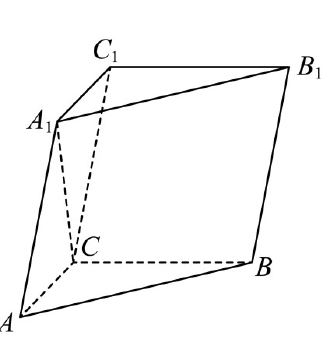
\includegraphics[width=\linewidth]{figures/2023_jia_li_q18.png}
\end{minipage}
\vspace{-1.8em}
\item（12分）

为探究某药物对小鼠的生长抑制作用，将$40$只小鼠均分为两组，分别为对照组（不加药物）和实验组（加药物）. 

\subq{（1）}{设其中两只小鼠中对照组小鼠数目为$X$，求$X$的分布列和数学期望；}

\subq{（2）}{测得$40$只小鼠体重如下（单位：g）：（已按从小到大排好）
对照组：
\begin{center}
17.3 18.4 20.1 20.4 21.5 23.2 24.6 24.8 25.0 25.4

26.1 26.3 26.4 26.5 26.8 27.0 27.4 27.5 27.6 28.3    
\end{center}


实验组：
\begin{center}

5.4 6.6 6.8 6.9 7.8 8.2 9.4 10.0 10.4 11.2

14.4 17.3 19.2 20.2 23.6 23.8 24.5 25.1 25.2 26.0
\end{center}
}

\subq{（i）}{求$40$只小鼠体重的中位数$m$，并完成下面$2\times2$列联表：\begin{tightcenter}
{\renewcommand{\arraystretch}{0.9}
\begin{tabular}{|c|c|c|}
\hline & $<m$ & $\geq m$ \\\hline
对照组 & & \\\hline
实验组 & & \\\hline
\end{tabular}}
\end{tightcenter}
}
\subq{（ii）}{根据$2\times2$列联表，能否有$95\%$的把握认为药物对小鼠生长有抑制作用. 
参考数据：
\begin{tightcenter}
{\renewcommand{\arraystretch}{0.9}
\begin{tabular}{|c|c|c|c|}
\hline $k_0$ & $0.10$ & $0.05$ & $0.010$ \\\hline
$P(K^2\geq k_0)$ & $2.706$ & $3.841$ & $6.635$ \\\hline
\end{tabular}}
\end{tightcenter}
}

\item（12分）

已知直线$x-2y+1=0$与抛物线$C:y^2=2px(p>0)$交于$A,B$两点，且$|AB|=4\sqrt{15}$. 

\subq{（1）}{求$p$；}

\subq{（2）}{设$C$的焦点为$F$，$M,N$为$C$上两点，且$\vec{MF}\cdot\vec{NF}=0$，求$\triangle MNF$面积的最小值.}

\item（12分）

已知$f(x)=ax-\dfrac{\sin x}{\cos^3x}$，$x\in\left(0,\dfrac\pi2\right)$. 

\subq{（1）}{若$a=8$，讨论$f(x)$的单调性；}

\subq{（2）}{若$f(x)<\sin 2x$恒成立，求$a$的取值范围.}
\end{examanswers}

\vspace{1em}
\begin{examanswers}[start=22]
\item（10分）【选修4-4：坐标系与参数方程】

已知$P(2,1)$，直线$l:$\linsys{x=2+t\cos\alpha,\\y=1+t\sin\alpha}（$t$为参数），$\alpha$为$l$的倾斜角，$l$与$x$轴、$y$轴正半轴交于$A,B$两点，且$|PA|\cdot|PB|=4$. 

\subq{（1）}{求$\alpha$的值；}

\subq{（2）}{以原点为极点，$x$轴正半轴为极轴建立极坐标系，求$l$的极坐标方程.}

\item（10分）【选修4-5：不等式选讲】

已知$f(x)=2|x-a|-a$，$a>0$. 

\subq{（1）}{求不等式$f(x)<x$的解集；}

\subq{（2）}{若曲线$y=f(x)$与$x$轴所围成的图形的面积为$2$，求$a$.}
\end{examanswers}

\end{document}
